\documentclass[fr]{../../../../../../eplexam}

\hypertitle{Théorie et algorithmique des graphes}{5}{INMA}{1691}{2017}{Janvier}{Majeure}
{Etudiants MAP de 2017\and Gilles Peiffer}
{Vincent Blondel et Jean-Charles Delvenne}

\section{}

\begin{enumerate}
	\item Considérez le graphe de co-présence,
	qui relie deux personnes
	si leurs intervalles de présence dans la bibliothèque s’intersectent,
	et qui est 2-connexe dans notre cas.
	Démontrez qu’un groupe de personnes forme une clique dans le graphe
	si et seulement si ces personnes se sont retrouvées ensemble
	au même moment dans la bibliothèque.
	\item Démontrez que l’ensemble des personnes présentes dans la pièce
	à un moment entre le départ de l’ambassadeur
	et l’arrivée de son épouse,
	forme une coupe de noeuds du graphe.
	Déduisez qu’il y a deux voleurs au minimum,
	car nul n’aurait pu ouvrir le coffre-fort
	et le refermer sans se faire remarquer
	des autres personnes présentes dans la pièce,
	qui sont dès lors complices.
	Bien sûr, l’ambassadeur et son épouse sont au-dessus de tout soupçon.
	\item Montrez que si un groupe de personnes
	forme une couverture de sommets
	alors au moins une des ces personnes est coupable.
	\item Qui sont les coupables?
	On estime que le Recteur, le Baron et l'amie intime
	ne sont pas coupables.

\end{enumerate}

\begin{figure}[h]
	\centering
	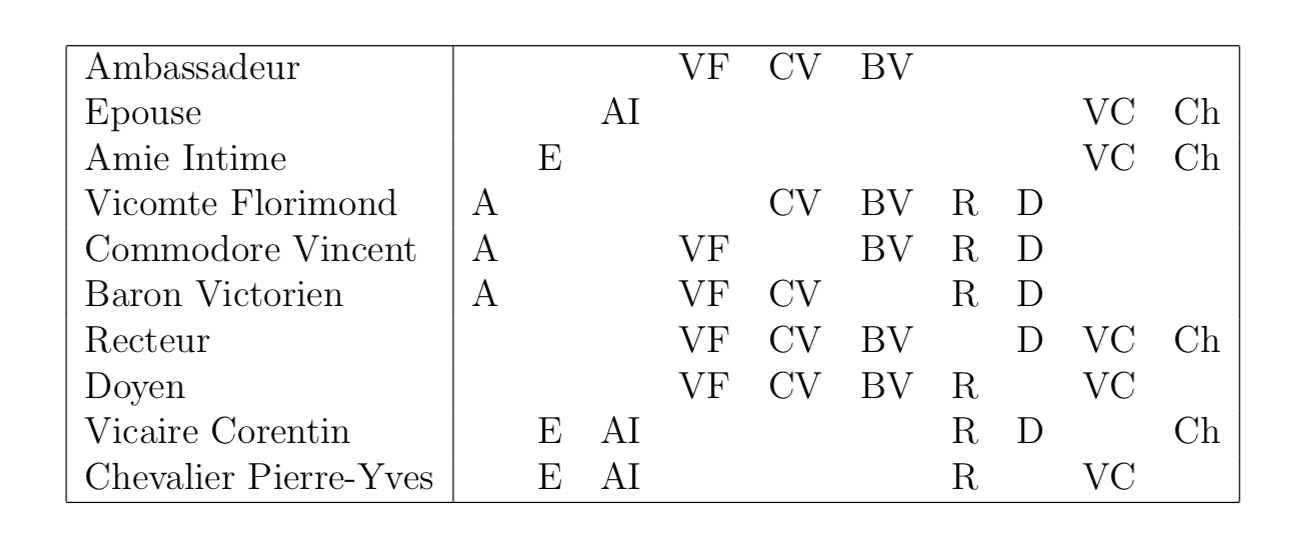
\includegraphics[scale=0.5]{img/presence}
\end{figure}

\begin{solution}

\begin{enumerate}

	\item Pour chaque personne $i$
	correspondant à un n\oe{}ud de la clique,
	on définit $a_i$ comme l'heure d'arrivée
	et $b_i$ comme l'heure de départ.
	Comme les n\oe{}uds forment une clique,
	on a $\forall i,j \quad a_i\leq b_j$ et donc il existe $t$
	tel que toutes les personnes de la clique sont présentes en même temps
	(prendre $t$ tel que $\max_i a_i \leq t \leq \min_i b_i$).

	\item Une coupe d'un graphe est un ensemble d'arêtes
	tel qu'il n'y ait plus aucun chemin d'un n\oe{}ud source
	vers un n\oe{}ud puits quand on retire cet ensemble du graphe.
	Ici, le n\oe{}ud source est l'ambassadeur
	(qui arrive et part en premier)
	et le noeud puits est l'épouse (qui arrive en dernière).
	Donc, l'ensemble des personnes arrivant
	entre le départ de l'ambassadeur et l'arrivée de l'épouse
	permet de supprimer tout chemin entre le n\oe{}ud source
	et le n\oe{}ud puits.
	Pour prouver qu'il y a au minimum 2 voleurs,
	il faut s'intéresser à la coupe minimum de notre graphe.
	En visualisant le graphe, nous voyons que R et D sont présents
	pour 2 groupes de personnes différents.
	Il suffit donc de prendre comme coupe
	les arêtes reliant Ch et VC à R et D et nous avons notre coupe minimum.

	\item Pour rappel, un ensemble indépendant d'un graphe
	est un ensemble de sommets qui ne sont pas adjacents entre eux.
	Le complémentaire de cet ensemble est appelé la couverture de sommets.

	On a prouvé à la question précédente qu'il y avait au moins 2 voleurs,
	qui étaient donc ensemble dans la bibliothèque pendant le vol;
	il y a donc une arête qui les relie.
	Une couverture devant couvrir l'ensemble des arêtes du graphe,
	et vu qu'il existe une arête entre les 2 (ou plus) voleurs,
	alors il faut qu'au moins un des voleurs soit dans la couverture.

	\item On peut voir que seuls VC et Ch forment une coupe
	qui ne contienne une personne de confiance. Ce sont eux les coupables.
\end{enumerate}

\end{solution}

\section{}
Emilie, 2 ans, a fait un beau dessin pour son père sur le thème de Noël.
Il s’agit d’une courbe fermée.
Cette courbe et ses nombreuses auto-intersections (en nombre fini tout de même)
divisent la feuille en un nombre fini de parties.
Henri (4 ans) et Guillaume (7 ans) veulent l’enjoliver davantage
en coloriant chaque partie de la feuille en bleu ou en rouge,
de sorte à ce que deux parties adjacentes (séparées par un arc de courbe)
ne soient jamais de la même couleur.
Le père se propose de rédiger un question d’examen sur ce thème.
Démontrez ce théorème des deux couleurs:
quelle que soit la courbe fermée d’Emilie,
ses deux frères pourront réaliser leur dessin.

\begin{solution}

On construit le graphe dual: un n\oe{}ud est une face sur la courbe,
deux n\oe{}uds sont reliés si leurs faces correspondantes sont adjacentes.
À chaque intersection, on a un nombre pair de chemins qui partent,
sinon ce ne serait pas une courbe fermée.
À chaque fois qu'on rajoute une intersection,
on rajoute une paire de chemins;
le graphe dual total/final n'a donc pas de cycle de longueur impaire.
Il est donc biparti et ainsi il est $2$-coloriable.

\end{solution}

\section{}

\begin{enumerate}
	\item L’Espagnol veut placer ses troupes en embuscade dans les cols
	pour réduire au maximum la longueur du front ennemi
	sans risquer de laisser la route vers Madrid ouverte.
	Modéliser le problème dans le langage de la théorie des graphes.

	\item Résolvez le problème: quels cols (arêtes) sont à défendre?

	\item Si les Français prennent un col aux Espagnols,
	ceux-ci doivent immédiatement se redéployer
	de façon à former un nouveau front minimal.
	Le col à défendre en priorité est donc
	celui qui donnerait le front le plus difficile à défendre,
	si pris par les Français.
	Proposez une méthode pour déterminer, dans votre solution,
	le col à défendre en priorité.

	\item Appliquez votre méthode:
	quel col (arête) est à défendre en priorité?

\end{enumerate}

\begin{figure}[h]
	\centering
	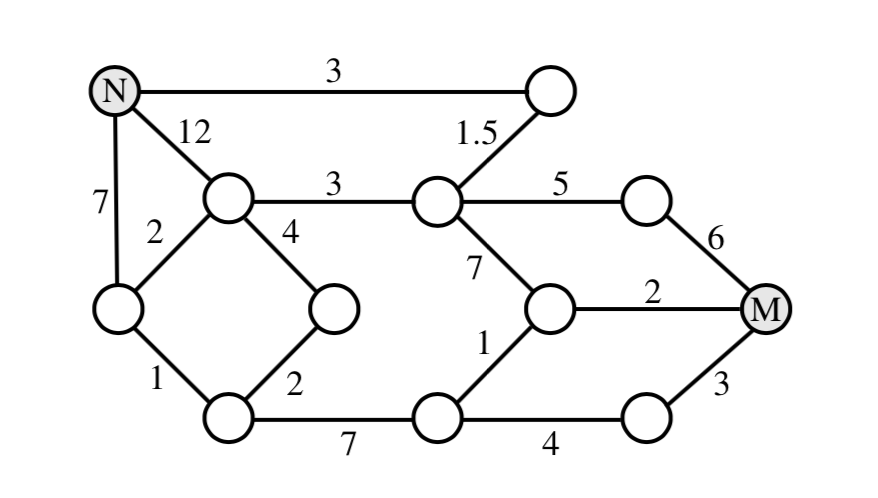
\includegraphics[scale=0.4]{img/flot}
	\caption{Graphe relatif à la question 3.}
	\label{fig:my_label}
\end{figure}

\begin{solution}

\begin{enumerate}

	\item Nous avons un problème de flots.
	Les n\oe{}uds sources sont les troupes de Napoléon,
	et le n\oe{}ud puits est Madrid,
	le point d'arrivée et l'objectif de ces troupes.
	L'Espagnol veut créer une embuscade
	afin de réduire au maximum la grandeur du front de Napoléon.
	Chaque route aura alors une capacité
	dédiée au nombre maximum de troupes qu'elle peut accueillir.
	Nous essaierons de trouver une coupe minimum
	afin d'obtenir le flot maximum de ce problème de théorie des graphes.

	\item Il suffit de prendre l'arête de poids $1.5$,
	celle de $3$ en dessous d'elle,
	et celles de $1$ et $2$ en bas du losange.
	Si on calcule le flot maximum,
	on se rend compte qu'il est bien égal à $7.5$.
	Il existe une technique pour récupérer le Min-Cut
	une fois qu'on a fait le Max-Flow:
	tous les n\oe{}uds que la source peut encore atteindre
	via des arêtes non saturées sont dans $S$,
	le reste est dans son complémentaire, $\bar{S}$.

	\item Si l'arête $uv$ est prise,
	on recalcule le Min-Cut en mettant le noeud $v$ dans $S$.
	On fait ceci pour toutes les arêtes de la coupe minimum,
	et on défend en priorité le col donnant le pire Min-Cut
	si l'arête qui y est adjacente dans la coupe
	est prise par les Espagnols.

	\item Dans ce cas-ci, le procédé indique
	que le col à défendre en priorité est soit
	celui adjacent à l'arête de poids $3$ dans la coupe trouvée ci-dessus,
	soit celui adjacent à l'arête de poids $1.5$.
	Dans les deux cas, la nouvelle coupe minimale devient
	les trois arêtes incidentes au n\oe{}ud M, pour un flot maximum de $11$.
\end{enumerate}

\end{solution}

\section{Vrai ou faux}

\begin{enumerate}

	\item Tout graphe $G$ admettant un couplage parfait
	est tel que
	\[
	\abs{\bigcup_{s\in S} \mathrm{Voisins}(s)} \geq \abs{S}
	\]
	pour tout ensemble de n\oe{}uds $S$.

	\item Tout graphe $G$ tel que
	$\abs{\bigcup_{s\in S} \mathrm{Voisins}(s)} \geq \abs{S}$
	pour tout ensemble de n\oe{}uds $S$ admet un couplage parfait.

	\item Tout graphe eulérien connexe est $2$-arête-connexe.

	\item Tout graphe biparti $k$-régulier connexe, pour $k > 1$,
	est $2$-arête-connexe.

	\item Tout graphe $3$-régulier a un nombre pair de n\oe{}uds.

	\item Bonus. Pour tout coloriage des points du plan en $3$ couleurs,
	il y a deux points de même couleur
	séparés par une distance unité (exactement).

\end{enumerate}

\begin{solution}

\begin{enumerate}

	\item VRAI. Comme il admet un couplage parfait,
	tout sommet est au moins connecté à un autre via le couplage.
	Donc, si on considère un ensemble $S$ de sommets,
	comme ils ont tous au moins un voisin,
	l'inégalité est prouvée.

	\item FAUX. $K_3$ par exemple.

	\item VRAI. C'est un graphe eulérien,
	il passe donc par chaque arête une et une seule fois et forme un cycle.
	Si on enlève une arête,
	on casse le cycle mais pas la connexité.
	Il faut enlever deux arêtes pour la casse.

	\item VRAI. Si le graphe est biparti et $k$-régulier avec $k > 1$,
	enlever une arête ne peut pas déconnecter le graphe.

	\item VRAI. On sait que $\sum d(v) = 2 \abs{E(G)}$
	et donc ici $3n = 2e$.
	On peut remarquer que $2e$ sera pair pour toutes les valeurs de $e$.
	Il faut donc que le produit $3n$ soit pair pour tout $n$.
	On peut enfin remarquer que c'est le cas pour les valeurs paires de $n$.

	\item VRAI. Un exemple de graphe distance-unité simple
	est le graphe de Golomb, représenté à la \figuref{golomb},
	qui ne peut pas être colorié avec moins de \(4\) couleurs.
	Dans ce graphe, les points à distance unité sont reliés par une arête.
	Un autre exemple est le graphe de Moser.

	\begin{figure}[H]
		\centering
		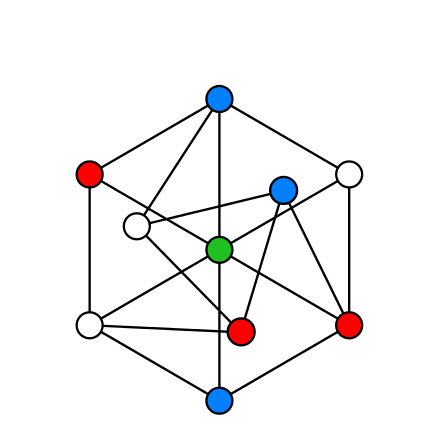
\includegraphics[width=0.5\textwidth]{img/golomb}
		\caption{Le graphe de Golomb.}
		\label{fig:golomb}
	\end{figure}

\end{enumerate}

\end{solution}

\end{document}
